\subsubsubsection{Interlayer}

This component is responsible of the communication between
different layers. Namely, the one which it belongs (the \textbf{middleware}) and
the \textbf{application}
layer, which uses the middleware layer.

The architecture of this application is depicted
in Figure \ref{fig:mw-interlayer}.

\begin{figure}[H]
  \centering
  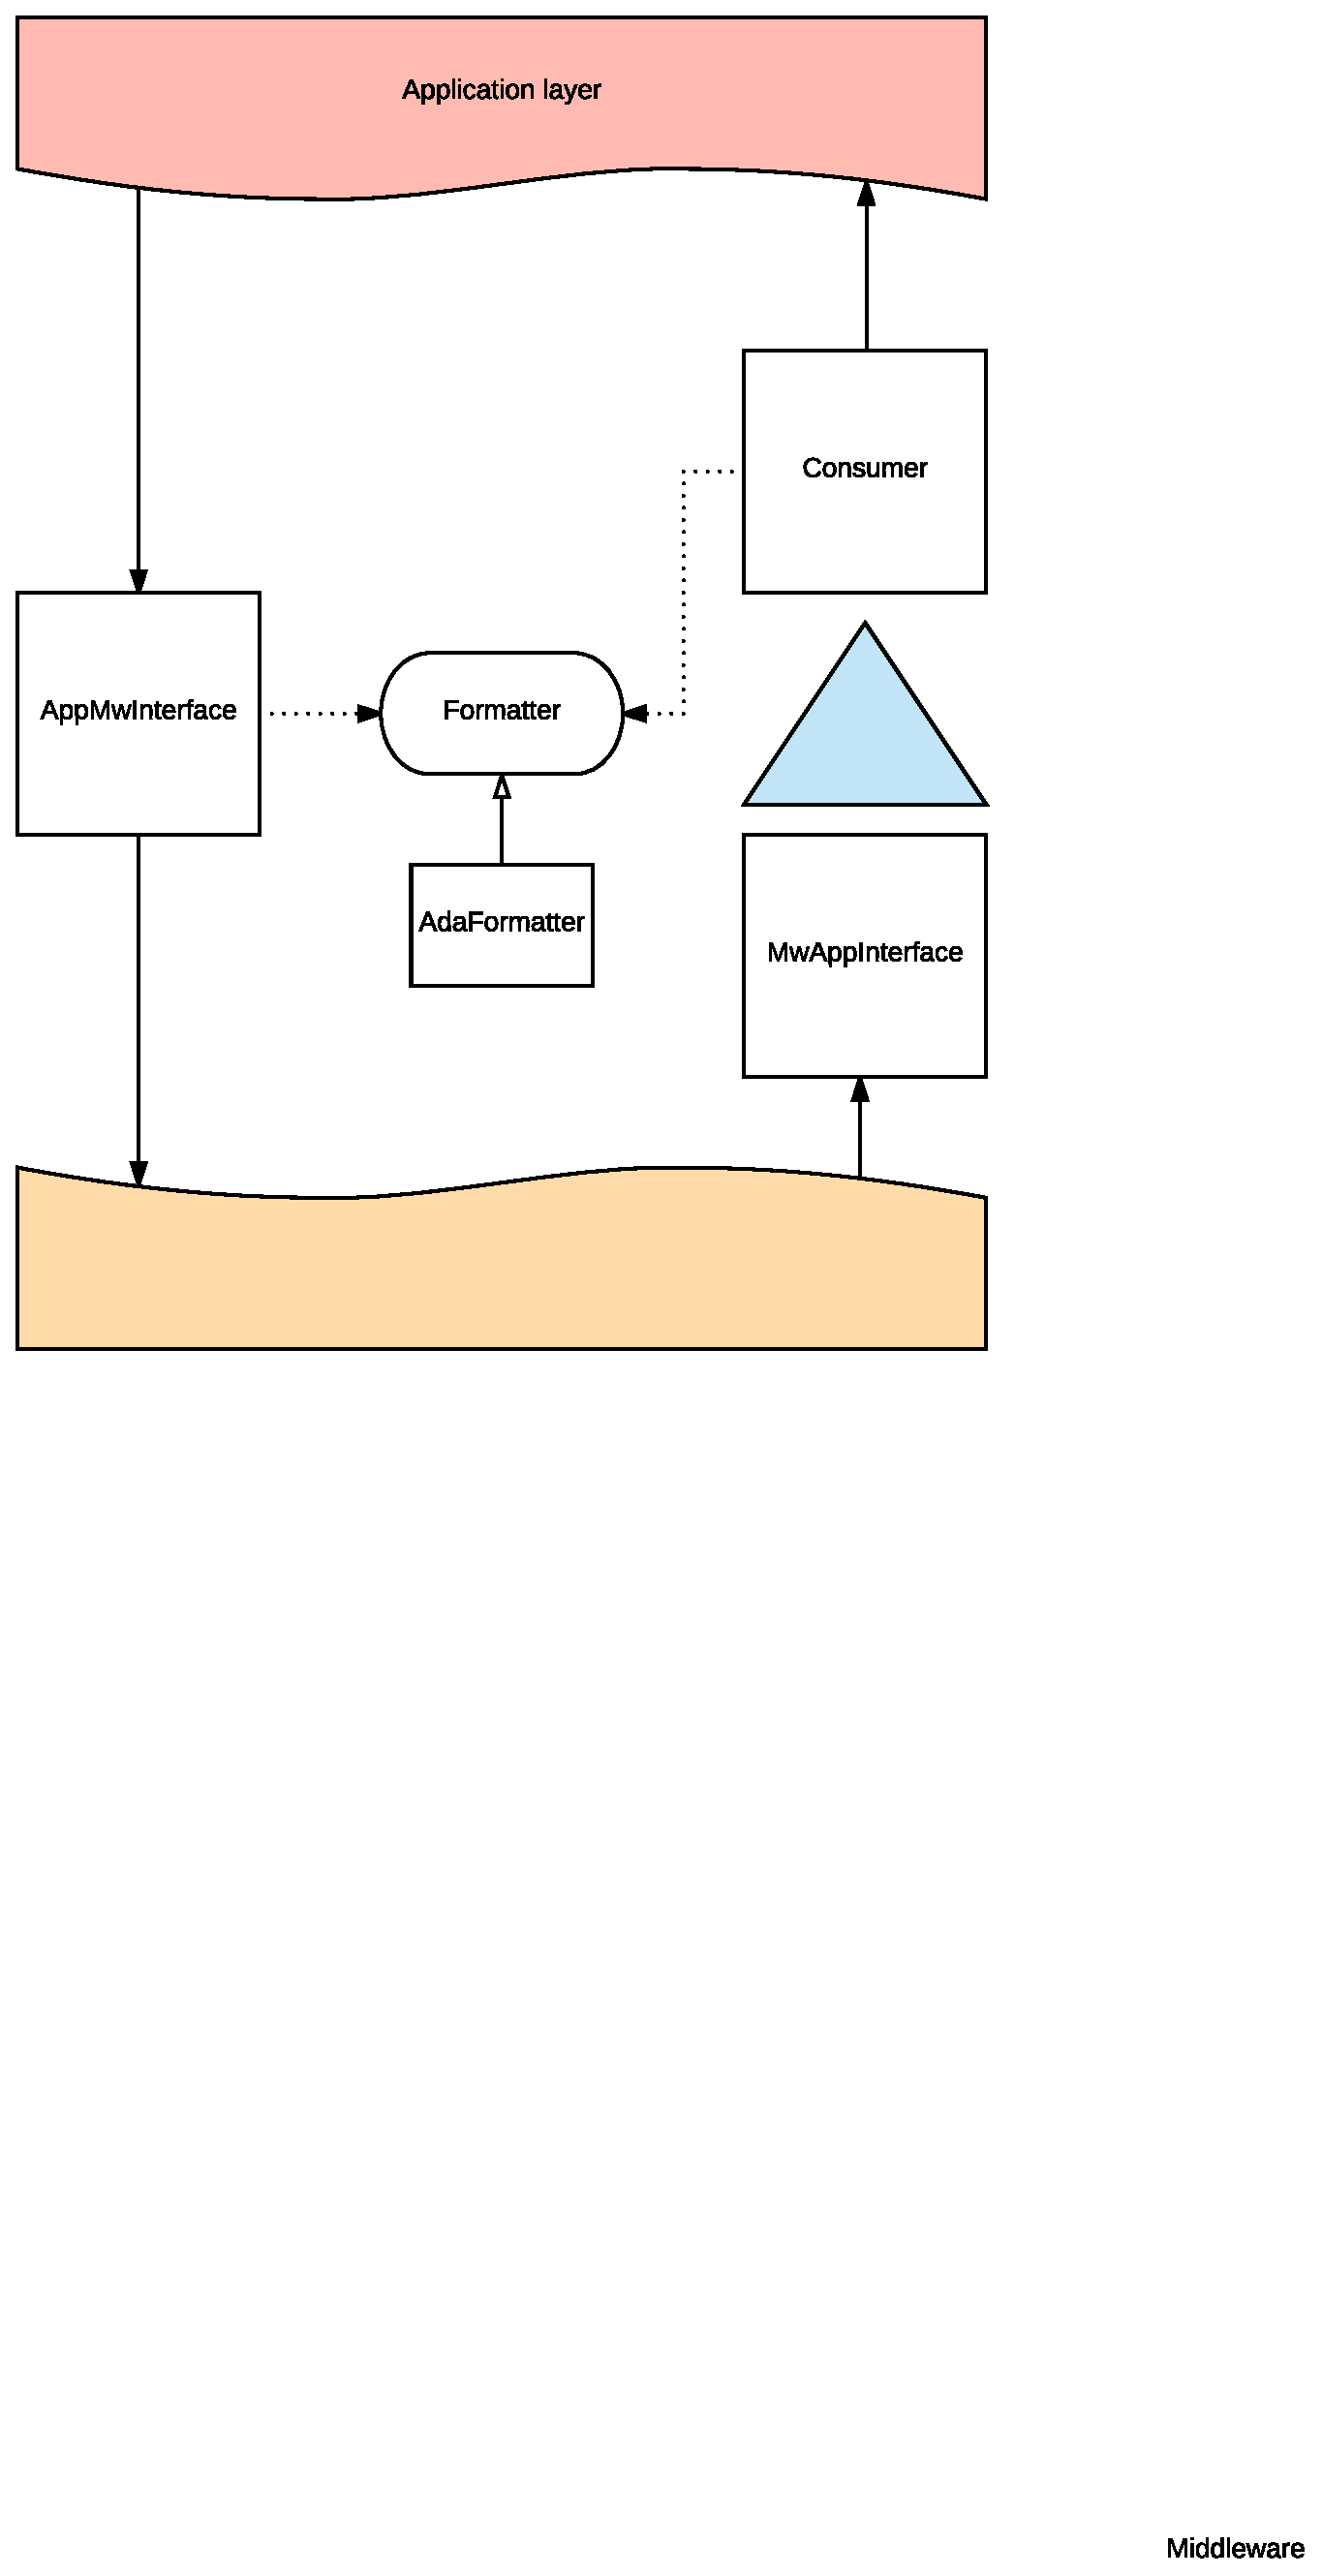
\includegraphics[height=12cm]{images/solution/mw/int/architect.eps}
  \caption{Middleware's Interlayer application}
  \label{fig:mw-interlayer}
\end{figure}

We can see that the Interlayer application embodies two flows of information, each
one directed in the opposite direction as the other (the orange band represents
the middleware).
\begin{itemize}
\item \textit{AppMwInterface} : listens on a port waiting for messages
from the application layer and passes them to other middleware applications.
It can receive several messages in parallel.

\item \textit{MwAppInterface} : receives requests from other
middleware applications.
Instead of blocking the requesting process
on the delivery of the message, it stores the message
in a Redis map of pending requests. Then, the request is
asynchronously handed over to the \textit{Consumer} module by means of the
GenStage behavior. The \textit{Consumer} instances send
pending messages to the application layer and, for each successful delivery,
pop the delivered messages from the Redis map.

\item \textit{Consumer} : can store meta-information for messages delivered to
the application. They do so in order to keep track of the RPCs performed by the
application layer. This is achieved by storing the id of the node which issued a
request in a Redis map. Then, when an RPC gets satisfied from the
application layer, \textit{AppMwInterface} correlates the answer with the
node which initially issued the request, and forwards the RPC result to it.
This feature allows us to preserve the transparency offered by the
middleware for application-level RPCs.

\end{itemize}
